\chapter{Relativistic Free Scalar Matter\label{AppFreeSca}}
%%%%%%%%%%%%%%%%%%%%%%%%%%%%%%%%%%%%%%%%%%%%%%%%%%%%%%%%%%%%%%%%%%%%%%%%%%%%%%%%%%%%%%%%%
In this appendix we discuss the kernels for relativistic free massless and massive scalar matter. Although free theories are somewhat trivial, these examples will allow us to discuss some of the differences between the quantum and the semiclassical kernels.
%%%%%%%%%%%%%%%%%%%%%%%%%%%%%%%%%%%%%%%%%%%%%%%%%%%%%%%%%%%%%%%%%%%%%%%%%%%%%%%%%%%%%%%%%
\section{Massive Scalar Particle}
%%%%%%%%%%%%%%%%%%%%%%%%%%%%%%%%%%%%%%%%%%%%%%%%%%%%%%%%%%%%%%%%%%%%%%%%%%%%%%%%%%%%%%%%%
After fixing the worldline reparametrization gauge symmetry with the choice $v = 1$, the action functional for a free massive scalar particle is
\begin{equation}
	S[q] = \int \mathrm{d}\tau \left[- \frac{1}{2} \dot{q}^{2} + \frac{1}{2}m^{2} \right] \qquad m > 0 \label{SmFree}
\end{equation}
where the range of the worldline parameter $\tau$ is
\begin{equation}
	{- \frac{T}{2} } < \tau < \frac{T}{2}
\end{equation}
with $T > 0$. The quantum kernel $\mathcal{F}$ is
\begin{equation}
	\mathcal{F}(O | I) = \int\limits_{0}^{\infty} \mathrm{d}T \int\limits_{x_{I}}^{x_{O}} \mathrm{D}q(\tau) \exp{\left(- i S[q] \right)}
\end{equation}
We will first calculate the semiclassical kernel, and then discuss the differences between the (exact) quantum kernel and the semiclassical kernel.
%%%%%%%%%%%%%%%%%%%%%%%%%%%%%%%%%%%%%%%%%%%%%%%%%%%%%%%%%%%%%%%%%%%%%%%%%%%%%%%%%%%%%%%%%
\subsection{Semiclassical Kernel}
%%%%%%%%%%%%%%%%%%%%%%%%%%%%%%%%%%%%%%%%%%%%%%%%%%%%%%%%%%%%%%%%%%%%%%%%%%%%%%%%%%%%%%%%%
In order to find the semiclassical kernel, we must first solve the classical equation of motion that follows from the action functional (\ref{SmFree}),
\begin{equation}
	\ddot{q} = 0
\end{equation}
subject to the boundary conditions
\begin{equation}
	q\left(- \frac{T}{2} \right) = x_{I}, \qquad q\left( \frac{T}{2} \right) = x_{O}
\end{equation}
The classical path $q_{*}$ is
\begin{equation}
	q_{*}(\tau) = \frac{x_{I} + x_{O}}{2} + (x_{O} - x_{I}) \left( \frac{\tau}{T} \right)
\end{equation}
Let $x \equiv x_{O} - x_{I}$. For a \textit{physical} massive particle we expect
\begin{equation}
	x^{2} < 0
\end{equation}
That is, the separation between the ``in'' position and the ``out'' position is a time-like spacetime interval.

We define the \textit{classical} conjugate momentum $p_{*}$ as
\begin{equation}
	p_{*}(\tau) \equiv \dot{q}_{*} = \frac{x}{T}
\end{equation}
This is a \textit{constant spacetime vector} that depends on the modulus $T$.

Evaluating the action functional (\ref{SmFree}) at the classical path yields the Van Vleck function,
\begin{equation}
	\Sigma \equiv S[q_{*}] = - \frac{1}{2 T} x^{2} + \frac{m^{2} T}{2}
\end{equation}
With the Van Vleck function, we can obtain the Van Vleck matrix,
\begin{equation}
	V_{mn} \equiv -i \frac{\partial^{2} \Sigma}{\partial x_{I}^{m} \partial x_{O}^{n}} = \left(- \frac{i}{T} \right) \eta_{mn}
\end{equation}
The semiclassical kernel $\mathcal{V}$ is
\begin{equation}
	\mathcal{V}(O | I) = \int\limits_{0}^{\infty} \mathrm{d}T \sqrt{- \det{(V)}} \exp{\left(- i \Sigma \right)}
\end{equation}
After evaluating the determinant of $V$, we find
\begin{equation}
	\mathcal{V}(O | I) = \int\limits_{0}^{\infty} \mathrm{d}T \left(- \frac{i}{T} \right)^{D/2} \exp{\left[ \frac{i}{2 T} x^{2} - \frac{i m^{2} T}{2} \right]} \label{Vx2}
\end{equation}
At first glance, this expression can be recognized as the \textit{exact} quantum kernel. However, the semiclassical kernel is only valid in the $\hbar \rightarrow 0$ limit. We are using units where $\hbar = 1$. If we had kept $\hbar$ explicit, there would had been factor of $\hbar$ dividing the Van Vleck function in the semiclassical kernel. In order to understand the consequences of the $\hbar \rightarrow 0$ limit, we make a change of variables
\begin{equation}
	T = \sqrt{-\frac{x^{2}}{m^{2}}} \omega
\end{equation}
Then, the semiclassical kernel becomes
\begin{equation}
\begin{split}
	\mathcal{V} = {}&{-i} \left(- i \sqrt{-\frac{m^{2}}{x^{2}}} \right)^{(D - 2)/2} \\
	&\times \int\limits_{0}^{\infty} \mathrm{d}\omega \left( \frac{1}{\omega} \right)^{D/2} \exp{\left[ -i \sqrt{- m^{2} x^{2}} \left( \frac{1}{2 \omega} + \frac{\omega}{2} \right) \right]}
\end{split} \label{VVKernIntegral}
\end{equation}
Thus, $\hbar \rightarrow 0$ is equivalent to the regime where $\sqrt{-m^{2}x^{2}} \rightarrow \infty$. Note that the latter limit allows two different cases,
\begin{equation}
	{-x^{2}} \rightarrow \infty, \qquad m^{2} \text{ fixed} \label{xLarge}
\end{equation}
or
\begin{equation}
	{-x^{2}} \text{ fixed}, \qquad m^{2} \rightarrow \infty \label{mLarge}
\end{equation}
The case (\ref{xLarge}) is consistent with the familiar intuition of having classical behavior (i.e. not quantum-mechanical) at long spacetime distances. Case (\ref{mLarge}) corresponds to a heavy scalar particle. In the semiclassical limit, we can integrate over $\omega$ with stationary methods. The stationary point is $\omega_{*} = 1$. At this stationary point, we have
\begin{equation}
	T_{*} = \sqrt{-\frac{x^{2}}{m^{2}}}
\end{equation}
Note that, at this value, the \textit{classical} conjugate momentum becomes
\begin{equation}
	p_{*}(\tau) = \frac{m x}{\sqrt{- x^{2}}} \quad \Longrightarrow \quad p_{*}^{2} + m^{2} = 0 \label{ccmOnShell}
\end{equation}
The ``in'' and ``out'' spacetime positions have components
\begin{equation}
	x_{I} = (t_{I}, \mathbf{x}_{I}) \qquad x_{O} = (t_{O}, \mathbf{x}_{O})
\end{equation}
with $t_{O} > t_{I}$. Thus,
\begin{equation}
	x^{2} = (x_{O} - x_{I})^{2} = -(t_{O} - t_{I})^{2} + (\mathbf{x}_{O} - \mathbf{x}_{I})^{2}
\end{equation}
We define the average spatial velocity vector $\mathbf{v}$ as
\begin{equation}
	\mathbf{v} \equiv \frac{\mathbf{x}_{O} - \mathbf{x}_{I}}{t_{O} - t_{I}}
\end{equation}
Thus, the components of the \textit{classical} conjugate momentum,
\begin{equation}
	p_{*} = (E, \mathbf{p})
\end{equation}
are given by
\begin{equation}
	E = \frac{m}{\sqrt{1 - \mathbf{v}^{2}}} \qquad \mathbf{p} = \frac{m \mathbf{v}}{\sqrt{1 - \mathbf{v}^{2}}}
\end{equation}
This are the familiar expressions for the energy $E$ and translational momentum $\mathbf{p}$ of a free massive relativistic particle. We can think of $T$ as parametrizing a family of worldlines. As part of the quantum theory, we must sum (i.e. integrate) over all possible values of $T$. Only the worldline with $T = T_{*}$ describes a truly classical (i.e. on-shell) relativistic particle.

After dealing with the integral over $\omega$, we find
\begin{equation}
	\mathcal{V} \approx {-\sqrt{2 \pi} i} \left(- i \sqrt{-\frac{m^{2}}{x^{2}}} \right)^{(D - 2)/2} \left( i \sqrt{-m^{2} x^{2}} \right)^{-1/2} \exp{\left[ -i \sqrt{- m^{2} x^{2}} \right]}
\end{equation}
which can be put in the form
\begin{equation}
	\mathcal{V} \approx -\frac{{\sqrt{2 \pi} i } m^{(D-2)}}{\left( i \sqrt{-m^{2} x^{2}} \right)^{(D - 1)/2}} \exp{\left[ -i \sqrt{- m^{2} x^{2}} \right]}
\end{equation}
%\begin{equation}
%	\mathcal{V} \approx {-\sqrt{2 \pi} i } m^{(D-2)} \left( i \sqrt{-m^{2} (x_{O} - x_{I})^{2}} \right)^{(1 - D)/2} \exp{\left[ -i \sqrt{- m^{2} (x_{O} - x_{I})^{2}} \right]} \nonumber
%\end{equation}
Another useful form follows after we write the exponential as an infinite sum,
\begin{equation}
	\mathcal{V} \approx {-\sqrt{2 \pi} i } m^{(D-2)} \sum_{n = 0}^{\infty} \frac{(-1)^{n}}{\Gamma(n+1)} (-2)^{y_{n}} \left( - \frac{2}{m^{2}x^{2}} \right)^{z_{n}} \label{VVKernFreem}
\end{equation}
where
\begin{equation}
	y_{n} \equiv \frac{1 - D}{4} + \frac{n}{2}, \qquad z_{n} \equiv -y_{n} = \frac{D - 1}{4} - \frac{n}{2} 
\end{equation}
Equation (\ref{VVKernFreem}) is our final result in the position basis.
%%%%%%%%%%%%%%%%%%%%%%%%%%%%%%%%%%%%%%%%%%%%%%%%%%%%%%%%%%%%%%%%%%%%%%%%%%%%%%%%%%%%%%%%%
\subsubsection{Fourier Transform}
%%%%%%%%%%%%%%%%%%%%%%%%%%%%%%%%%%%%%%%%%%%%%%%%%%%%%%%%%%%%%%%%%%%%%%%%%%%%%%%%%%%%%%%%%
Strictly speaking, the Fourier transform is a quantum device. By this, we mean that it involves $\hbar$. The $\hbar \rightarrow 0$ limit of the Fourier transform is the classical Legendre transform that switches between Hamiltonian and Lagrangian mechanics. This transform amounts to swapping $\dot{q}_{*}$ with $p_{*}$ defined by (\ref{ccmOnShell}). We found that $p_{*}$ is constant in $\tau$, so we have
\begin{equation}
	p_{I} = p_{O}
\end{equation}
We also found that $p_{*}$ satisfies the on-shell condition at $T = T_{*}$. So, as expected, the \textit{classical} momentum is conserved and on-shell.

However, nothing prevents us from taking a full Fourier transform of the semiclassical kernel $\mathcal{V}$. When we do this, the Fourier transform takes us to a \textit{quantum} momentum basis, and thus, the momentum variables are \textit{not} on-shell. The Fourier transform is
\begin{equation}
	\widehat{\mathcal{V}}(O|I) = \int \int \mathrm{d}x_{I} \mathrm{d}x_{O} \, \mathcal{V}(O|I) \exp{\left(i x_{I} \cdot p_{I} - i x_{O} \cdot p_{O} \right)}
\end{equation}
We first make a change of position variables,
\begin{equation}
	X \equiv \frac{x_{I} + x_{O}}{2} \qquad x \equiv x_{O} - x_{I}
\end{equation}
The corresponding conjugate momenta are
\begin{equation}
	P \equiv p_{O} - p_{I} \qquad p \equiv \frac{p_{I} + p_{O}}{2}
\end{equation}
such that
\begin{equation}
	x_{I} \cdot p_{I} - x_{O} \cdot p_{O} = - X \cdot P - x \cdot p
\end{equation}
Since $\mathcal{V}$ does not depend on $X$, the integral yields a Dirac delta:
\begin{equation}
	\int \mathrm{d}X \, \exp{\left( -i X \cdot P \right)} = \delta(P)
\end{equation}
The Dirac delta restricts to $P = 0$ or $p_{O} = p_{I}$. This means that the incoming momentum is equal to the outgoing momentum, a result expected from translation invariance. Then
\begin{equation}
	p = p_{I} = p_{O}
\end{equation}
We are left with the integral over $x$,
\begin{equation}
	\widehat{\mathcal{V}}(p) = \delta(P) \int \mathrm{d}x \, \mathcal{V}(x) \exp{\left( -i x \cdot p \right)}
\end{equation}
Using (\ref{VVKernFreem}) and Fourier-transforming each term in the sum yields
\begin{equation}
\begin{split}
	\widehat{\mathcal{V}}(p) = {}& {- \sqrt{2\pi} i} m^{D-2} \left( - \frac{1}{m^{2}} \right)^{D/2} \delta(P) \\
	&\times \sum_{n = 0}^{\infty} \frac{(-1)^{n}}{\Gamma(n + 1)} (-2)^{y_{n}} \frac{\Gamma(w_{n})}{\Gamma(z_{n})} \left( - \frac{2 m^{2}}{p^{2}} \right)^{w_{n}}
\end{split} \label{VVHatSum}
\end{equation}
with
\begin{equation}
	w_{n} \equiv \frac{D}{2} - z_{n} = \frac{D + 1}{4} + \frac{n}{2}
\end{equation}
We separate the sum in (\ref{VVHatSum}) into the part with even $n$ and the part with odd $n$,
\begin{equation}
	\widehat{\mathcal{V}}(p) = \widehat{\mathcal{V}}_{\text{even}}(p) + \widehat{\mathcal{V}}_{\text{odd}}(p)
\end{equation}
Each term can be evaluated separately,
\begin{align}
	\widehat{\mathcal{V}}_{\text{even}}(p) &= \frac{E_{D}}{m^{2}} \delta(P) \left(- \frac{m^{2}}{p^{2}} \right)^{(1 + D)/4} {}_{2} F_{1} \left( \frac{5 - D}{4}, \frac{1 + D}{4}; \frac{1}{2}; - \frac{m^{2}}{p^{2}}  \right) \label{VHatEven1} \\
	\widehat{\mathcal{V}}_{\text{odd}}(p) &=	\frac{O_{D}}{m^{2}} \delta(P) \left(- \frac{m^{2}}{p^{2}} \right)^{(3 + D)/4} {}_{2} F_{1} \left( \frac{7 - D}{4}, \frac{3 + D}{4}; \frac{3}{2}; - \frac{m^{2}}{p^{2}}  \right) \label{VHatOdd1}
\end{align}
with
\begin{equation}
	E_{D} \equiv - 2 \sqrt{\pi} i^{(D+1)} (-1)^{(1-D)/4} \frac{\Gamma\left( \frac{D + 1}{4} \right)}{\Gamma\left( \frac{D - 1}{4} \right)}
\end{equation}
and
\begin{equation}
	O_{D} \equiv - 4 \sqrt{\pi} i^{D} (-1)^{(1-D)/4} \frac{\Gamma\left( \frac{D + 3}{4} \right)}{\Gamma\left( \frac{D - 3}{4} \right)}
\end{equation}
%\begin{equation}
%	E_{D} \equiv 2 \sqrt{\pi} i^{(3D+5)/2} \frac{\Gamma\left( \frac{D + 1}{4} \right)}{\Gamma\left( \frac{D - 1}{4} \right)}
%\end{equation}
%and
%\begin{equation}
%	O_{D} \equiv 4 \sqrt{\pi} i^{(3D+7)/2} \frac{\Gamma\left( \frac{D + 3}{4} \right)}{\Gamma\left( \frac{D - 3}{4} \right)}
%\end{equation}
Recall the Pfaff identities,
\begin{align}
	{}_{2} F_{1}(a, b; c; x) &= \left( \frac{1}{1 - x} \right)^{a} {}_{2} F_{1} \left( a, c-b; c; \frac{x}{x - 1} \right) \label{Pfaffa} \\
	{}_{2} F_{1}(a, b; c; x) &= \left( \frac{1}{1 - x} \right)^{b} {}_{2} F_{1} \left( c - a, b; c; \frac{x}{x - 1} \right) \label{Pfaffb}
\end{align}
Combining both of these yields the Euler identity,
\begin{equation}
	{}_{2} F_{1}(a, b; c; x) = \left( \frac{1}{1 - x} \right)^{(a + b - c)} {}_{2} F_{1} \left(c - a, c - b; c; x \right) \label{EulerId}
\end{equation}
Using this identity, we find
\begin{align}
	{}_{2} F_{1} \left( \frac{5 - D}{4}, \frac{1 + D}{4}; \frac{1}{2}; - \frac{m^{2}}{p^{2}}  \right) &= \left( \frac{p^{2}}{m^{2} + p^{2}} \right) {}_{2} F_{1} \left( \frac{D - 3}{4}, \frac{1 - D}{4}; \frac{1}{2}; - \frac{m^{2}}{p^{2}}  \right) \nonumber \\
	{}_{2} F_{1} \left( \frac{7 - D}{4}, \frac{3 + D}{4}; \frac{3}{2}; - \frac{m^{2}}{p^{2}}  \right) &= \left( \frac{p^{2}}{m^{2} + p^{2}} \right) {}_{2} F_{1} \left( \frac{D - 1}{4}, \frac{3 - D}{4}; \frac{3}{2}; - \frac{m^{2}}{p^{2}}  \right) \nonumber
\end{align}
So then, (\ref{VHatEven1}) and (\ref{VHatOdd1}) become
\begin{align}
	\widehat{\mathcal{V}}_{\text{even}} &= -\frac{E_{D}}{m^{2} + p^{2}} \delta(P) \left(- \frac{m^{2}}{p^{2}} \right)^{(D - 3)/4} {}_{2} F_{1} \left( \frac{D - 3}{4}, \frac{1 - D}{4}; \frac{1}{2}; - \frac{m^{2}}{p^{2}}  \right) \label{VHatEven2} \\
	\widehat{\mathcal{V}}_{\text{odd}} &=	 -\frac{O_{D}}{m^{2} + p^{2}} \delta(P) \left(- \frac{m^{2}}{p^{2}} \right)^{(D - 1)/4} {}_{2} F_{1} \left( \frac{D - 1}{4}, \frac{3 - D}{4}; \frac{3}{2}; - \frac{m^{2}}{p^{2}}  \right) \label{VHatOdd2}
\end{align}
In this form, the on-shell singularity at $p^{2} + m^{2} = 0$ appears as a common overall factor.
%%%%%%%%%%%%%%%%%%%%%%%%%%%%%%%%%%%%%%%%%%%%%%%%%%%%%%%%%%%%%%%%%%%%%%%%%%%%%%%%%%%%%%%%%
\subsubsection{One-Dimensional Kernel}
%%%%%%%%%%%%%%%%%%%%%%%%%%%%%%%%%%%%%%%%%%%%%%%%%%%%%%%%%%%%%%%%%%%%%%%%%%%%%%%%%%%%%%%%%
The one-dimensional kernel is somewhat trivial, but it will play a role later, so we discuss it now. In the position basis we have
\begin{equation}
	\mathcal{V}(x) = - \frac{\sqrt{2 \pi} i}{m} \exp{\left[ - i \sqrt{- m^{2} x^{2}} \right]} \label{VleckPropaX1}
\end{equation}
All the $x$-dependence appears in the exponential. Note that the $m \rightarrow 0$ limit is not well-defined

Setting $D = 1$ yields
\begin{equation}
	E_{1} = 0  \qquad O_{1} = 2i
\end{equation}
We also have
\begin{align}
	\lim_{D \rightarrow 1} \left[ \left(- \frac{m^{2}}{p^{2}} \right)^{(D - 3)/4} {}_{2} F_{1} \left( \frac{D - 3}{4}, \frac{1 - D}{4}; \frac{1}{2}; - \frac{m^{2}}{p^{2}}  \right) \right] &= \sqrt{- \frac{p^{2}}{m^{2}}} \\
	\lim_{D \rightarrow 1} \left[ \left(- \frac{m^{2}}{p^{2}} \right)^{(D - 1)/4} {}_{2} F_{1} \left( \frac{D - 1}{4}, \frac{3 - D}{4}; \frac{3}{2}; - \frac{m^{2}}{p^{2}}  \right) \right] &= 1
\end{align}
Thus, in the momentum basis we have
\begin{equation}
	\widehat{\mathcal{V}}(p) = \left[ -\frac{2i}{m^{2} + p^{2}} \right] \delta(P)
\end{equation}
which coincides with the familiar Feynman propagator for a massive scalar particle.
%%%%%%%%%%%%%%%%%%%%%%%%%%%%%%%%%%%%%%%%%%%%%%%%%%%%%%%%%%%%%%%%%%%%%%%%%%%%%%%%%%%%%%%%%
\subsubsection{Three-Dimensional Kernel}
%%%%%%%%%%%%%%%%%%%%%%%%%%%%%%%%%%%%%%%%%%%%%%%%%%%%%%%%%%%%%%%%%%%%%%%%%%%%%%%%%%%%%%%%%
The three-dimensional kernel will also play a role later. In the position basis we have
\begin{equation}
	\mathcal{V}(x) = - \frac{\sqrt{2 \pi} }{\sqrt{- x^{2}}} \exp{\left[ - i \sqrt{- m^{2} x^{2}} \right]} \label{VleckPropaX3}
\end{equation}
This is the Minkowski analog of the Yukawa potential. Note that the $m \rightarrow 0$ limit is well-defined,
\begin{equation}
	\lim_{m \rightarrow 0} \mathcal{V}(x) = - \frac{\sqrt{2 \pi} }{\sqrt{- x^{2}}} \label{VleckX3M0}
\end{equation}
Indeed, $D = 3$ is the \textit{only} case for which the semiclassical kernel has a well-defined massless limit.

Setting $D = 3$ yields
\begin{equation}
	E_{3} = 2i \qquad O_{3} = 0
\end{equation}
We also have
\begin{align}
	\lim_{D \rightarrow 3} \left[ \left(- \frac{m^{2}}{p^{2}} \right)^{(D - 3)/4} {}_{2} F_{1} \left( \frac{D - 3}{4}, \frac{1 - D}{4}; \frac{1}{2}; - \frac{m^{2}}{p^{2}}  \right) \right] &= 1 \\
	\lim_{D \rightarrow 3} \left[ \left(- \frac{m^{2}}{p^{2}} \right)^{(D - 1)/4} {}_{2} F_{1} \left( \frac{D - 1}{4}, \frac{3 - D}{4}; \frac{3}{2}; - \frac{m^{2}}{p^{2}}  \right) \right] &= \sqrt{- \frac{m^{2}}{p^{2}}}
\end{align}
Thus, in the momentum basis we have
\begin{equation}
	\widehat{\mathcal{V}}(p) = \left[ -\frac{2i}{m^{2} + p^{2}} \right] \delta(P)
\end{equation}
which also coincides with the familiar Feynman propagator.
%%%%%%%%%%%%%%%%%%%%%%%%%%%%%%%%%%%%%%%%%%%%%%%%%%%%%%%%%%%%%%%%%%%%%%%%%%%%%%%%%%%%%%%%%
\subsubsection{Four-Dimensional Kernel}
%%%%%%%%%%%%%%%%%%%%%%%%%%%%%%%%%%%%%%%%%%%%%%%%%%%%%%%%%%%%%%%%%%%%%%%%%%%%%%%%%%%%%%%%%
In $D = 1$ and $D = 3$ we found that the semiclassical kernel in the momentum basis coincides with the traditional Feynman propagator. Indeed, these two cases are the only cases for which this is true. Since in this dissertation we will work with four-dimensional theories, we now turn to the case when $D = 4$. In the position basis we have
\begin{equation}
	\mathcal{V}(x) = -\frac{{\sqrt{2 \pi} i } m^{2}}{\left( i \sqrt{-m^{2} (x_{O} - x_{I})^{2}} \right)^{3/2}} \exp{\left[ -i \sqrt{- m^{2} (x_{O} - x_{I})^{2}} \right]} \label{VleckPropaX4}
\end{equation}
This corresponds to a higher-dimensional analog of the Yukawa potential.

Setting $D = 4$ yields
\begin{equation}
	E_{4} = 2 \sqrt{\pi} (-1)^{3/4} \frac{\Gamma\left(\frac{5}{4}\right)}{\Gamma\left(\frac{3}{4}\right)} \qquad O_{4} = 4 \sqrt{\pi} (-1)^{1/4} \frac{\Gamma\left(\frac{7}{4}\right)}{\Gamma\left(\frac{1}{4}\right)}
\end{equation}
Unlike in $D = 1$ or $D = 3$, both the even and odd parts will contribute to the semiclassical kernel in the momentum basis:
\begin{align}
	\widehat{\mathcal{V}}_{\text{even}}(p) &= -\frac{E_{4}}{m^{2} + p^{2}} \delta(P) \left(- \frac{m^{2}}{p^{2}} \right)^{1/4} {}_{2} F_{1} \left( \frac{1}{4}, -\frac{3}{4}; \frac{1}{2}; - \frac{m^{2}}{p^{2}}  \right) \\
	\widehat{\mathcal{V}}_{\text{odd}}(p) &=	 -\frac{O_{4}}{m^{2} + p^{2}} \delta(P) \left(- \frac{m^{2}}{p^{2}} \right)^{3/4} {}_{2} F_{1} \left( \frac{3}{4}, -\frac{1}{4}; \frac{3}{2}; - \frac{m^{2}}{p^{2}}  \right)
\end{align}
We write
\begin{equation}
	\widehat{\mathcal{V}}(p) = W(\xi) \left[ -\frac{2i}{m^{2} + p^{2}} \right] \delta(P), \qquad \xi \equiv - \frac{p^{2}}{m^{2}} \label{VleckP4}
\end{equation}
with
\begin{equation}
	W(\xi) = \frac{E_{4}}{2i} \left( \frac{1}{\xi} \right)^{1/4} {}_{2} F_{1} \left( \frac{1}{4}, -\frac{3}{4}; \frac{1}{2}; \frac{1}{\xi}  \right) + \frac{O_{4}}{2i} \left( \frac{1}{\xi} \right)^{3/4} {}_{2} F_{1} \left( \frac{3}{4}, -\frac{1}{4}; \frac{3}{2}; \frac{1}{\xi}  \right) \nonumber
\end{equation}
Figures \ref{ReW4Fig} and \ref{ImW4Fig} display the real and imaginary parts of $W(\xi)$.

\begin{figure}
\centering
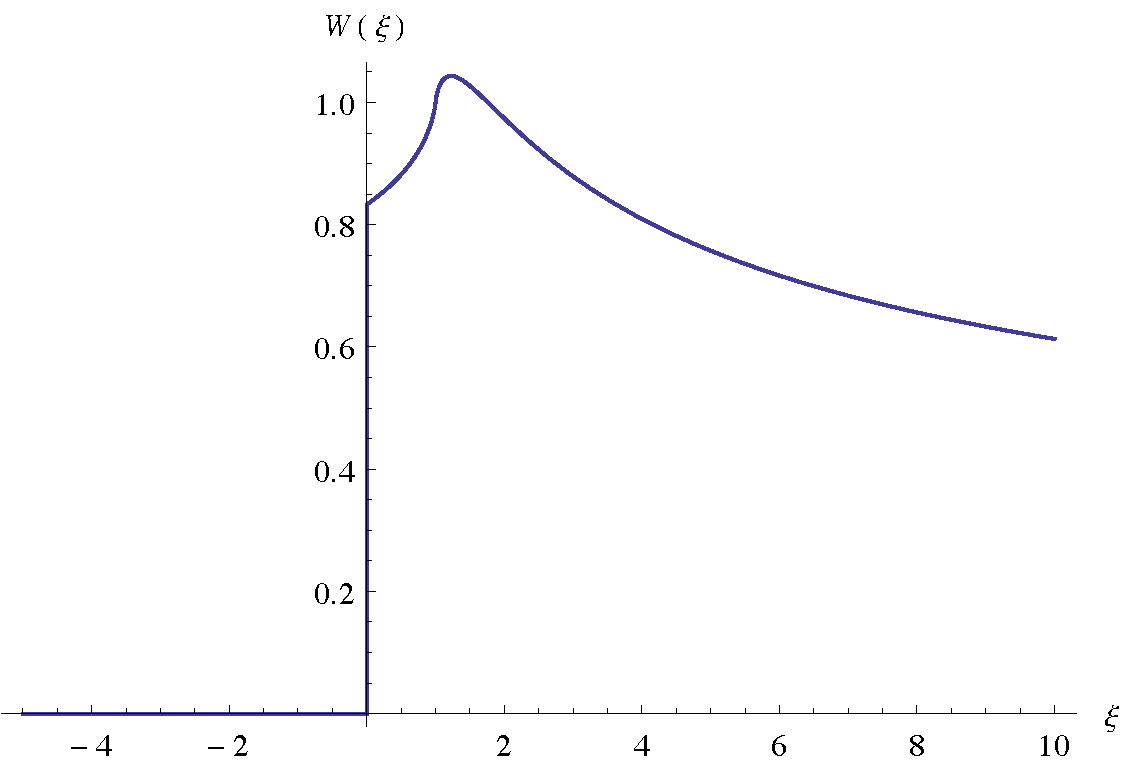
\includegraphics[scale=0.6]{Plots/ReW4.pdf}
\caption[Real part of $W(\xi)$]{Real part of $W(\xi)$.}
\label{ReW4Fig}
\end{figure}

\begin{figure}
\centering
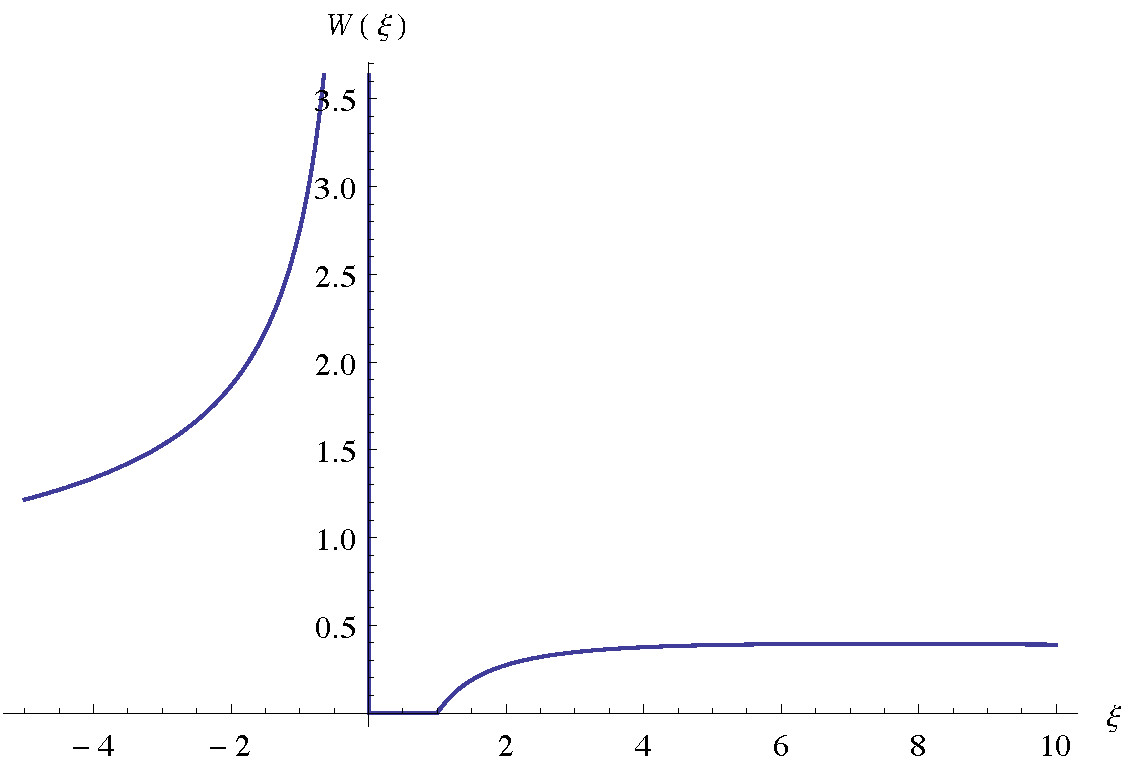
\includegraphics[scale=0.6]{Plots/ImW4.pdf}
\caption[Imaginary part of $W(\xi)$]{Imaginary part of $W(\xi)$.}
\label{ImW4Fig}
\end{figure}

Note that on-shell we have $\xi = 1$ and
\begin{equation}
	\operatorname{Re}{[W(1)]} = 1 \qquad \operatorname{Im}{[W(1)]} = 0
\end{equation}
Far away from the origin we have
\begin{equation}
	\operatorname{Re}{[W(\infty)]} = \operatorname{Im}{[W(\infty)]} = 0
\end{equation}
As we discussed earlier, there are two limits that are equivalent to the $\hbar \rightarrow 0$ limit. In limit (\ref{xLarge}), we have $-x^{2} \rightarrow \infty$, which corresponds to $-p^{2} \rightarrow 0$. On the other hand, in limit (\ref{mLarge}) we have $m^{2} \rightarrow \infty$. Both of these limits are equivalent to the $\xi \rightarrow 0$ limit.
%%%%%%%%%%%%%%%%%%%%%%%%%%%%%%%%%%%%%%%%%%%%%%%%%%%%%%%%%%%%%%%%%%%%%%%%%%%%%%%%%%%%%%%%%
\subsection{Quantum Kernel}
%%%%%%%%%%%%%%%%%%%%%%%%%%%%%%%%%%%%%%%%%%%%%%%%%%%%%%%%%%%%%%%%%%%%%%%%%%%%%%%%%%%%%%%%%
The quantum kernel can be found by evaluating the integral in (\ref{VVKernIntegral}) with exact methods. The outcome involves a modified Bessel function of the second kind,
\begin{equation}
	\mathcal{F}(x) = -2i \left(- i \sqrt{-\frac{m^{2}}{x^{2}}} \right)^{(D - 2)/2} K_{(D-2)/2} \left[ i \sqrt{- m^{2} x^{2}} \right] \label{FBesselK}
\end{equation}
This is the familiar Feynman propagator in the position basis.
%%%%%%%%%%%%%%%%%%%%%%%%%%%%%%%%%%%%%%%%%%%%%%%%%%%%%%%%%%%%%%%%%%%%%%%%%%%%%%%%%%%%%%%%%
\subsubsection{Fourier Transform}
%%%%%%%%%%%%%%%%%%%%%%%%%%%%%%%%%%%%%%%%%%%%%%%%%%%%%%%%%%%%%%%%%%%%%%%%%%%%%%%%%%%%%%%%%
To change to the momentum basis, we perform a Fourier transform,
\begin{equation}
	\widehat{\mathcal{F}}(p) = \delta(P) \int \mathrm{d}x \, \mathcal{F}(x) \exp{\left( - i x \cdot p \right)}
\end{equation}
Instead of using the complicated expression from above, we go back to (\ref{Vx2}). After integrating over $x$, we find
\begin{equation}
	\widehat{\mathcal{F}}(p) = \delta(P) \int\limits_{0}^{\infty} \mathrm{d}T \, \exp{\left[ - T \left( -\frac{p^{2} + m^{2}}{2i} \right) \right]}
\end{equation}
which, after integration over $T$, yields
\begin{equation}
	\widehat{\mathcal{F}}(p) = \left[ - \frac{2i}{m^{2} + p^{2}} \right] \delta(P) \label{FeynPropa}
\end{equation}
Thus, the exact quantum kernel has the expected simple form in the momentum basis.
%%%%%%%%%%%%%%%%%%%%%%%%%%%%%%%%%%%%%%%%%%%%%%%%%%%%%%%%%%%%%%%%%%%%%%%%%%%%%%%%%%%%%%%%%
\subsubsection{One-Dimensional Kernel}
%%%%%%%%%%%%%%%%%%%%%%%%%%%%%%%%%%%%%%%%%%%%%%%%%%%%%%%%%%%%%%%%%%%%%%%%%%%%%%%%%%%%%%%%%
Setting $D = 1$ in (\ref{FBesselK}) yields
\begin{equation}
	\mathcal{F}(x) = - \frac{\sqrt{2 \pi} i}{m} \exp{\left[ - i \sqrt{- m^{2} x^{2}} \right]}
\end{equation}
which coincides with the corresponding semiclassical kernel (\ref{VleckPropaX1}). This explains why in the momentum basis, the semiclassical kernel coincides with the Feynman propagator (\ref{FeynPropa}). We can say that in $D = 1$ the semiclassical kernel is \textit{exact}.
%%%%%%%%%%%%%%%%%%%%%%%%%%%%%%%%%%%%%%%%%%%%%%%%%%%%%%%%%%%%%%%%%%%%%%%%%%%%%%%%%%%%%%%%%
\subsubsection{Three-Dimensional Kernel}
%%%%%%%%%%%%%%%%%%%%%%%%%%%%%%%%%%%%%%%%%%%%%%%%%%%%%%%%%%%%%%%%%%%%%%%%%%%%%%%%%%%%%%%%%
Setting $D = 3$ in (\ref{FBesselK}) yields
\begin{equation}
	\mathcal{F}(x) = - \frac{\sqrt{2 \pi}}{\sqrt{-x^{2}}} \exp{\left[ - i \sqrt{- m^{2} x^{2}} \right]}
\end{equation}
which also coincides with the corresponding semiclassical kernel (\ref{VleckPropaX3}). This explains why in the momentum basis, the semiclassical kernel coincides with the Feynman propagator (\ref{FeynPropa}). This means that in $D = 3$ the semiclassical kernel is also \textit{exact}. Indeed, $D = 1$ and $D = 3$ are the \textit{only} cases for which this statement is true.
%%%%%%%%%%%%%%%%%%%%%%%%%%%%%%%%%%%%%%%%%%%%%%%%%%%%%%%%%%%%%%%%%%%%%%%%%%%%%%%%%%%%%%%%%
\subsubsection{Four-Dimensional Kernel}
%%%%%%%%%%%%%%%%%%%%%%%%%%%%%%%%%%%%%%%%%%%%%%%%%%%%%%%%%%%%%%%%%%%%%%%%%%%%%%%%%%%%%%%%%
Setting $D = 4$ in (\ref{FBesselK}) yields
\begin{equation}
	\mathcal{F}(x) = - \frac{2 m}{\sqrt{-x^{2}}} K_{1}\left[ i \sqrt{- m^{2} x^{2}} \right]
\end{equation}
which differs considerably from the corresponding semiclassical kernel (\ref{VleckPropaX4}). However, as $\sqrt{-m^{2} x^{2}} \rightarrow \infty$ we can use the asymptotic expansion
\begin{equation}
	K_{\nu}(z) \sim \frac{1}{2} \sqrt{\frac{2\pi}{z}} \exp{(-z)}
\end{equation}
to obtain (\ref{VleckPropaX4}). So we find that in $D = 4$ the semiclassical kernel agrees with the quantum kernel in either the large spacetime distance or large mass limit. Because of Fourier-Heisenberg conjugacy, large $-x^{2}$ corresponds to small $-p^{2}$. Indeed, besides the simple pole when $p^{2} + m^{2} = 0$, the imaginary part of the semiclassical kernel (\ref{VleckP4}) has a singularity when $p^{2} = 0$.
%%%%%%%%%%%%%%%%%%%%%%%%%%%%%%%%%%%%%%%%%%%%%%%%%%%%%%%%%%%%%%%%%%%%%%%%%%%%%%%%%%%%%%%%%
\section{Massless Scalar Particle}
%%%%%%%%%%%%%%%%%%%%%%%%%%%%%%%%%%%%%%%%%%%%%%%%%%%%%%%%%%%%%%%%%%%%%%%%%%%%%%%%%%%%%%%%%
We cannot repeat the analysis from the previous section for the case of a free massless scalar particle and expect to obtain valid results. As we already saw, the semiclassical kernel in the position basis corresponds to either the large spacetime distance limit or the large mass limit. Both of these regimes are not valid for massless particles, which travel along null spacetime intervals ($x^{2} = 0$) and are, well, massless ($m = 0$). For completeness we discuss the exact quantum kernel.

Setting $m = 0$ in (\ref{Vx2}) leads to
\begin{align}
	\mathcal{F}(x) &= \int\limits_{0}^{\infty} \mathrm{d}T \left(- \frac{i}{T} \right)^{D/2} \exp{\left[ \frac{i}{2 T} x^{2} \right]} \nonumber \\
	&= -i \Gamma\left( \frac{D - 2}{2} \right) \left( \frac{2}{x^{2}} \right)^{(D - 2)/2}
\end{align}
Note that for $D = 3$ this coincides with the massless limit of the massive quantum/semiclassical kernels obtained in (\ref{VleckX3M0}).